\documentclass{standalone}
\usepackage{tikz}
\usetikzlibrary{patterns, positioning}
\usepackage[sfdefault]{ClearSans} %% option 'sfdefault' activates Clear Sans as the default text font
\usepackage[T1]{fontenc}

\begin{document}
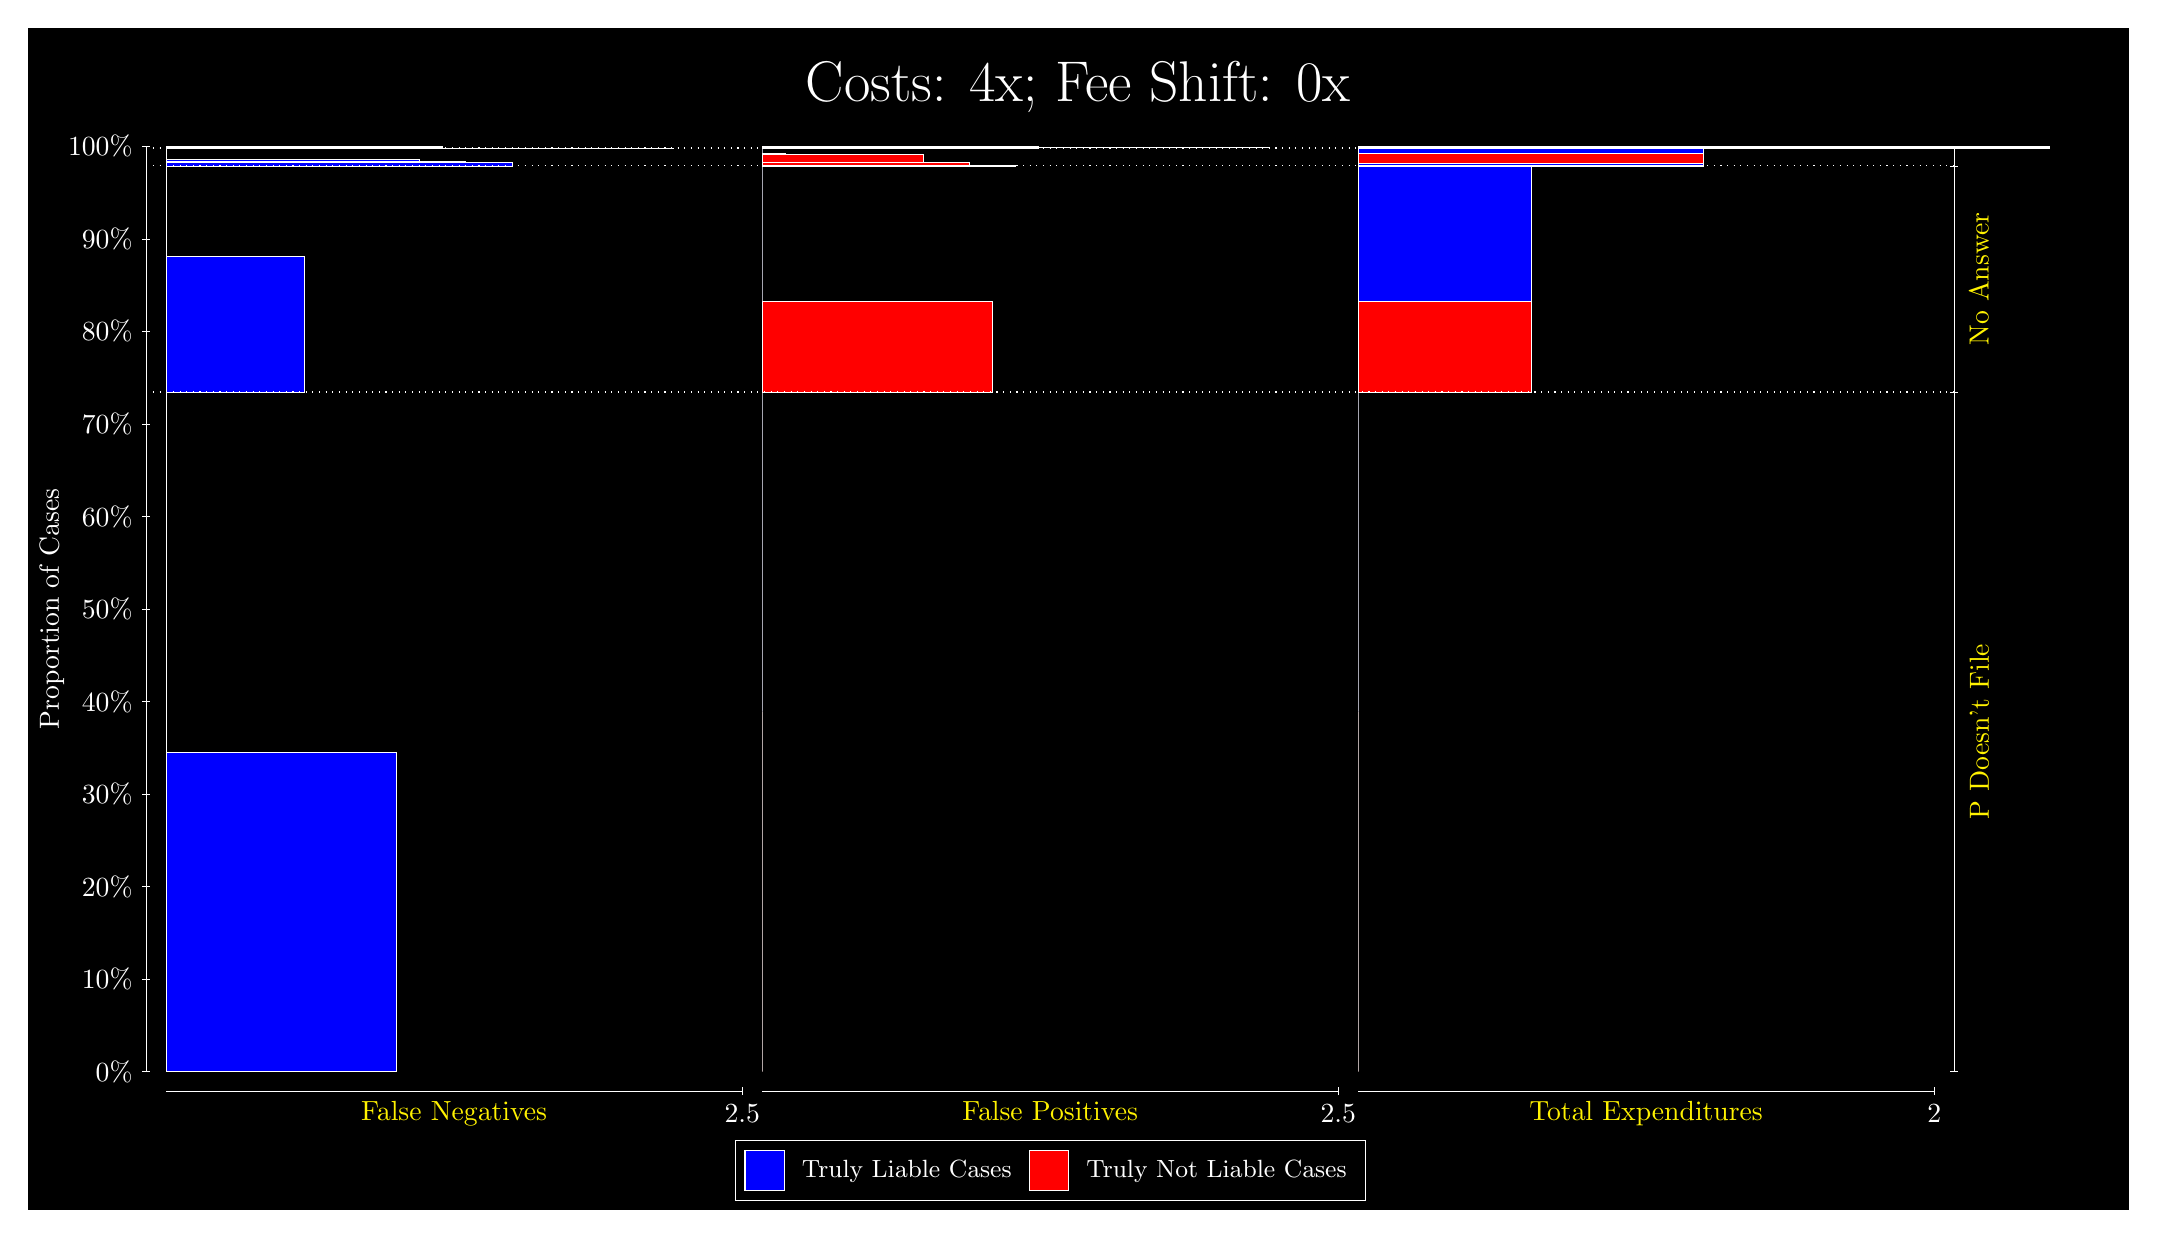
\begin{tikzpicture}
\draw[fill=black] (0,0) rectangle (26.667,15);
\draw[text=white] (0,13.5) rectangle (26.667,15) node[midway] {\huge Costs: 4x; Fee Shift: 0x};
\draw[white, very thin] (1.5,1.75) -- (1.5,13.5);
\node[rotate=90, text=white, anchor=center] at (0.3, 7.625) {Proportion of Cases};
\draw[white, very thin] (1.45,1.75) -- (1.55,1.75);
\node[text=white, anchor=east] at (1.45, 1.75) {0\%};
\draw[white, very thin] (1.45,2.925) -- (1.55,2.925);
\node[text=white, anchor=east] at (1.45, 2.925) {10\%};
\draw[white, very thin] (1.45,4.1) -- (1.55,4.1);
\node[text=white, anchor=east] at (1.45, 4.1) {20\%};
\draw[white, very thin] (1.45,5.275) -- (1.55,5.275);
\node[text=white, anchor=east] at (1.45, 5.275) {30\%};
\draw[white, very thin] (1.45,6.45) -- (1.55,6.45);
\node[text=white, anchor=east] at (1.45, 6.45) {40\%};
\draw[white, very thin] (1.45,7.625) -- (1.55,7.625);
\node[text=white, anchor=east] at (1.45, 7.625) {50\%};
\draw[white, very thin] (1.45,8.8) -- (1.55,8.8);
\node[text=white, anchor=east] at (1.45, 8.8) {60\%};
\draw[white, very thin] (1.45,9.975) -- (1.55,9.975);
\node[text=white, anchor=east] at (1.45, 9.975) {70\%};
\draw[white, very thin] (1.45,11.15) -- (1.55,11.15);
\node[text=white, anchor=east] at (1.45, 11.15) {80\%};
\draw[white, very thin] (1.45,12.325) -- (1.55,12.325);
\node[text=white, anchor=east] at (1.45, 12.325) {90\%};
\draw[white, very thin] (1.45,13.5) -- (1.55,13.5);
\node[text=white, anchor=east] at (1.45, 13.5) {100\%};

\draw[white, very thin] (24.457,1.75) -- (24.457,13.5);
\draw[white, very thin] (24.407,1.75) -- (24.507,1.75);
\node[anchor=west] at (24.407, 1.75) {};
\draw[white, very thin] (24.407,10.38) -- (24.507,10.38);
\node[anchor=west] at (24.407, 10.38) {};
\draw[white, very thin] (24.407,13.251) -- (24.507,13.251);
\node[anchor=west] at (24.407, 13.251) {};
\draw[white, very thin] (24.407,13.475) -- (24.507,13.475);
\node[anchor=west] at (24.407, 13.475) {};
\draw[white, very thin] (24.407,13.485) -- (24.507,13.485);
\node[anchor=west] at (24.407, 13.485) {};
\draw[white, very thin] (24.407,13.5) -- (24.507,13.5);
\node[anchor=west] at (24.407, 13.5) {};

\draw[white, very thin, fill=blue] (1.75,1.75) rectangle (4.6775,5.8089);
\draw[white, very thin, fill=red] (1.75,5.8089) rectangle (1.75,10.38);
\draw[white, very thin, fill=blue] (1.75,10.38) rectangle (3.5065,12.1);
\draw[white, very thin, fill=red] (1.75,12.1) rectangle (1.75,13.251);
\draw[white, very thin, fill=blue] (1.75,13.251) rectangle (6.1413,13.302);
\draw[white, very thin, fill=blue] (1.75,13.302) rectangle (5.5558,13.316);
\draw[white, very thin, fill=blue] (1.75,13.316) rectangle (4.9703,13.332);
\draw[white, very thin, fill=red] (1.75,13.332) rectangle (1.75,13.475);
\draw[white, very thin, fill=blue] (1.75,13.475) rectangle (8.1906,13.479);
\draw[white, very thin, fill=red] (1.75,13.479) rectangle (1.75,13.485);
\draw[white, very thin, fill=blue] (1.75,13.485) rectangle (5.2631,13.496);
\draw[white, very thin, fill=red] (1.75,13.496) rectangle (1.75,13.5);
\draw[white, very thin, fill=red] (9.3189,1.75) rectangle (9.3189,6.3207);
\draw[white, very thin, fill=blue] (9.3189,6.3207) rectangle (9.3189,10.38);
\draw[white, very thin, fill=red] (9.3189,10.38) rectangle (12.246,11.531);
\draw[white, very thin, fill=blue] (9.3189,11.531) rectangle (9.3189,13.251);
\draw[white, very thin, fill=red] (9.3189,13.251) rectangle (12.539,13.264);
\draw[white, very thin, fill=red] (9.3189,13.264) rectangle (11.954,13.295);
\draw[white, very thin, fill=red] (9.3189,13.295) rectangle (11.368,13.394);
\draw[white, very thin, fill=blue] (9.3189,13.394) rectangle (9.6116,13.41);
\draw[white, very thin, fill=blue] (9.3189,13.41) rectangle (9.3189,13.475);
\draw[white, very thin, fill=red] (9.3189,13.475) rectangle (12.832,13.481);
\draw[white, very thin, fill=blue] (9.3189,13.481) rectangle (9.9044,13.485);
\draw[white, very thin, fill=red] (9.3189,13.485) rectangle (15.759,13.489);
\draw[white, very thin, fill=blue] (9.3189,13.489) rectangle (12.832,13.5);
\draw[white, very thin, fill=red] (16.888,1.75) rectangle (16.888,6.3207);
\draw[white, very thin, fill=blue] (16.888,6.3207) rectangle (16.888,10.38);
\draw[white, very thin, fill=red] (16.888,10.38) rectangle (19.083,11.531);
\draw[white, very thin, fill=blue] (16.888,11.531) rectangle (19.083,13.251);
\draw[white, very thin, fill=red] (16.888,13.251) rectangle (21.279,13.264);
\draw[white, very thin, fill=blue] (16.888,13.264) rectangle (21.279,13.279);
\draw[white, very thin, fill=red] (16.888,13.279) rectangle (21.279,13.41);
\draw[white, very thin, fill=blue] (16.888,13.41) rectangle (21.279,13.475);
\draw[white, very thin, fill=red] (16.888,13.475) rectangle (25.67,13.481);
\draw[white, very thin, fill=blue] (16.888,13.481) rectangle (25.67,13.485);
\draw[white, very thin, fill=red] (16.888,13.485) rectangle (25.67,13.489);
\draw[white, very thin, fill=blue] (16.888,13.489) rectangle (25.67,13.5);
\draw[white, dotted] (1.5,10.38) -- (24.457,10.38);
\draw[white, dotted] (1.5,13.251) -- (24.457,13.251);
\draw[white, dotted] (1.5,13.475) -- (24.457,13.475);
\draw[white, dotted] (1.5,13.485) -- (24.457,13.485);
\draw[white, very thin] (1.75,1.5) -- (9.0689,1.5);
\node[text=yellow, anchor=north] at (5.4094, 1.5) {False Negatives};
\draw[white, very thin] (9.0689,1.45) -- (9.0689,1.55);
\node[text=white, anchor=north] at (9.0689, 1.45) {2.5};

\draw[white, very thin] (9.3189,1.5) -- (16.638,1.5);
\node[text=yellow, anchor=north] at (12.978, 1.5) {False Positives};
\draw[white, very thin] (16.638,1.45) -- (16.638,1.55);
\node[text=white, anchor=north] at (16.638, 1.45) {2.5};

\draw[white, very thin] (16.888,1.5) -- (24.207,1.5);
\node[text=yellow, anchor=north] at (20.547, 1.5) {Total Expenditures};
\draw[white, very thin] (24.207,1.45) -- (24.207,1.55);
\node[text=white, anchor=north] at (24.207, 1.45) {2};

\node[text=yellow, centered, rotate=90] at (24.777, 6.0648) {P Doesn't File};
\node[text=yellow, centered, rotate=90] at (24.777, 11.815) {No Answer};




\draw (12.978300999999998,1.5) node[draw=none] (baseCoordinate) {};
\begin{scope}[align=center]
        \matrix[scale=0.5, draw=white, below=0.5cm of baseCoordinate, nodes={draw}, column sep=0.1cm]{
            \node[rectangle, draw, minimum width=0.5cm, minimum height=0.5cm, fill=blue] {}; &
            \node[draw=none, font=\small, text=white] (B) {Truly Liable Cases}; &
            \node[rectangle, draw, minimum width=0.5cm, minimum height=0.5cm, fill=red] {}; &
            \node[draw=none, font=\small, text=white] (B) {Truly Not Liable Cases}; \\
            };
\end{scope}

\end{tikzpicture}
\end{document}